\chapter{Herramientas utilizadas}
\label{herramientas}
En este capítulo se describen las tecnologías web que se han utilizado en este TFG. Para añadir la recogida de sondas a Unibotics se ha utilizado como tecnologías del lado del cliente HTML para dar estructura, CSS para el diseño y JavaScript para definir las acciones, las tecnologías del lado del servidor han sido el \textit{framework} de Django y base de datos SQL\footnote{Structured Query Language}.Se ha integrado una base de datos llamada Elasticsearch para la recogida de la información y como visualización de estadísticas automáticas se ha utilizado Dash.
\section{Tecnologías web}
En esta sección se hablará de las diferentes tecnologías que forman Unibotics, la plataforma web educativa donde se realiza este trabajo y las cuales han sido usadas para llevar acabo los objetivos de este.
\subsection{HTML}
HTML son las siglas de \textit{HyperText Markup Language} donde "HiperTexto" se refiere a un texto donde hay enlaces a otra página web o en la misma página permitiendo que los documentos estén interconectados entre sí, esto es una parte fundamental de la web. Con marcado hace referencia a que HTML define la estructura del documento por ejemplo que parte del documento va a ser un titulo y donde se va a encontrar y por último con lenguaje como ya hemos dicho anteriormente HTML es un lenguaje pero no de programación si no marcado.\\

La estructura de un documento HTML esta compuesto por la definición del tipo de documento con \textit{\textless!DOCTYPE html\textgreater}, el elemento  \textit{\textless html \textgreater} y \textit{\textless/html \textgreater} para dar comienzo y final al documento HTML, el elemento {\textless head \textgreater} y {\textless/head \textgreater} donde se introducen los metadatos como es el idioma del documento o el titulo que aparece en la pestaña de la página y el elemento {\textless body \textgreater} y {\textless/body \textgreater} donde se escribe todo el contenido que se quiere mostrar a los usuarios.\cite{html}

\begin{figure}[H]
    \centering
    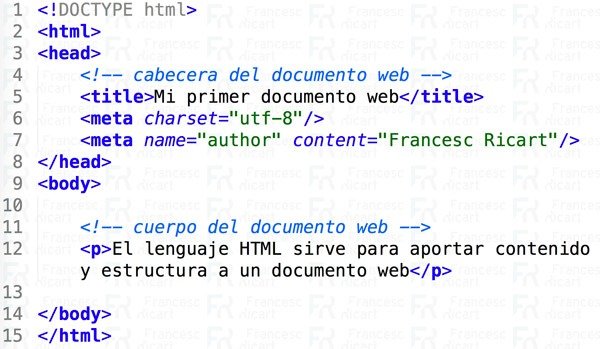
\includegraphics[width=9cm, keepaspectratio]{img/html.jpg}
    \caption{Estructura HTML}
    \label{fig:html}
\end{figure}

Un elemento de HTML esta compuesto por etiquetas que son palabras que marcan el inicio y final de una sección. La etiqueta de apertura esta formada por una palabra o letra rodeada por '\textless' y '\textgreater' dando comienzo al elemento y normalmente con una etiqueta de cierre al igual que la de la apertura pero rodeada por '\textless/' y '\textgreater'. La etiqueta no distingue entre mayúsculas y minúsculas. Aunque haya una gran cantidad de etiquetas a veces se necesita información adicional para completar los elementos, esto se consigue gracias a los atributos.\\ 

El atributo se encuentra dentro de la etiqueta de apertura con un espacio en blanco del nombre de la etiqueta o de otro atributo, el atributo esta compuesto por un nombre seguido del signo igual ( = ) y el valor del atributo entre comillas. \\

Cada etiqueta tiene unos atributos asociados y estos a la vez unos valores predefinidos si se da un valor erróneo a un atributo al renderizar la página esta lo ignorará. Algunos atributos son obligatorios como en el caso de las imágenes, vídeos o enlaces como se muestra en la figura\ref{fig:elemento}, la etiqueta para los enlaces es \textit{a} y es obligatorio que le siga el atributo \textit{href}  para poder añadir la dirección a la que va a dirigir dicho enlace. Entre las etiquetas de apertura y cierre nos encontramos con el texto que será el contenido de la sección.\cite{etiqueta}


\begin{figure}[H]
    \centering
    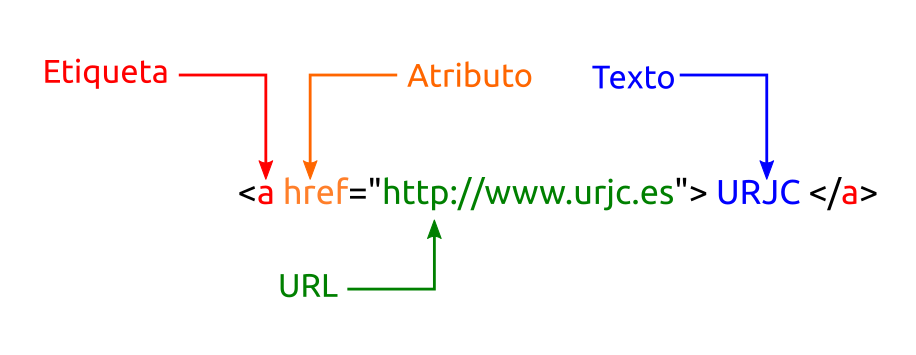
\includegraphics[width=12cm, keepaspectratio]{img/elemento.png}
    \caption{Estructura de un elemento HTML}
    \label{fig:elemento}
\end{figure}

Hay dos tipos de elementos, los elementos de bloques que son los elementos que ocupan toda una linea en el documento estos son los encabezados, listas o párrafos y los elementos en linea que solo ocupan el espacio de su contenido como los botones, enlaces o imágenes. Esto se puede cambiar gracias a atributos. Para estructurar el documento disponemos de dos etiquetas generales, \textit{\textless div \textgreater} la cual crea una sección de tipo bloque y \textit{\textless span \textgreater} para crear una sección en linea.\cite{juan2}

La última versión es la HTML5 la cual es utilizada en este proyecto, como mejoras respecto a anteriores versiones está la introducción de las etiquetas de audio \textit{\textless audio \textgreater} y vídeo \textit{\textless audio\textgreater}, anteriormente la web no estaba pensado para multimedia y había que meter parches como\textit{ Flash} de \textit{Adobe}. Se introduce SVG\footnote{Scalable Vector Graphics }para hacer gráficos vectoriales y así no se podrán ver los píxeles de las imágenes, también como novedad se tiene Canvas la cual es una web de diseño gráfico y composición de imágenes y WebGL que es una especie de Canvas pero en 3D. En HTML5 si das permiso incorpora una API\footnote{Application Programming Interfaces} de geolocalización donde se puede ver la ubicación y por último tambien incorpora lo denominado \textit{Drag and Drop} que consiste en arrastrar y soltar para facilitar la interacción con el usuario.\\

\newpage
\subsection{CSS}
CSS es el lenguaje de estilo encarga del diseño y presentación de los documentos HTML. Para llamar la atención de los usuarios en páginas web es importante añadir estilo a los documentos por eso se utiliza CSS, el cual puede definirse como un atributo de HTML llamado\textit{ style}, otra forma de meter estilo es utilizando la etiqueta {\textless style\textgreater} en la cabeza del documento HTML pero la mejor opción para añadir estilo es separándolo de la estructura, es decir, del documento HTML creando una hoja de estilo \textit{.css}  debido a que es más sencillo realizar cambios y se podrá diversificar el trabajo en estructura y estilo siendo más productivo. Para vincular la hoja de estilo con el HTML se utiliza la etiqueta \textit{\textless link\textgreater} en la cabecera.\\

La estructura de una regla CSS se divide en selectores que contienen pares de propiedad-valor como se muestra en la figura \ref{fig:css}. En los selectores se pone el nombre de las etiquetas las cuales quieres cambiar su estilo como puede ser la etiqueta \textit{body}, además estos selectores pueden ser el valor del atributo \textit{id} el cual es un identificador único para un elemento de HTML en este caso se pone el símbolo # antes del valor de su \textit{id}, a parte de identificar un elemento con un \textit{id} se puede utilizar el atributo \textit{class }que es un identificador para varios elementos, en este caso para añadirle estilo a los elementos pertenecientes a la misma clase al selector se le añade un punto delante.

\begin{figure}[H]
    \centering
    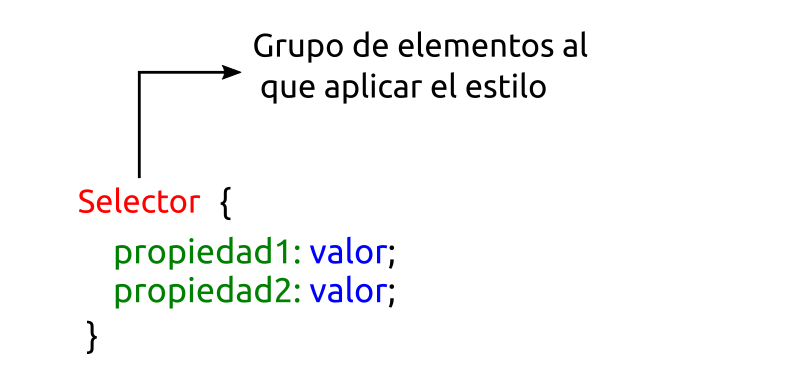
\includegraphics[width=12cm, keepaspectratio]{img/css.png}
    \caption{Sintaxis CSS}
    \label{fig:css}
\end{figure}
\newpage
Las propiedades indican cual es el estilo que se quiere cambiar en un elemento como puede ser el color o el tamaño. Cada propiedad tiene unos valores asociados que en algunas ocasiones sse pueden escribir de diferente manera como en el caso de los colores, se puede escribir directamente como \textit{red} o ponerlo en su valor hexadecimal o en valores RGB\footnote{ Red, Green, Blue,}.\\

A la hora de utilizar estilos se puede poner estilos contradictorios en este caso el último estilo definido será el que se acabe aplicando, esta sería la parte de cascada que indica las siglas CSS. Si se ha utilizado una hoja de estilo pero además se ha definido en una etiqueta HTML, el definido en la etiqueta será el utilizado al renderizar el documento. La herencia también es un concepto importante en CSS ya que si un elemento no tiene estilo pero esta contenido en otro elemento que si tiene, este heredará su estilo. Los identificadores únicos tendrán preferencia a añadir el estilo que los identificadores de clase, el nombre de la etiqueta como selector es el de menor preferencia entre los selectores.\cite{juan3}


\subsection{JavaScript}
JavaScript es un lenguaje de programación interpretado que permite la ejecución de código orientado a eventos.Pueden actuar sobre el navegador a través de objetos integrados como un botón. El DOM\footnote{Document Object Model}, API que representa al documento y define la manera de interactuar con él, puede ser modificado dinámicamente gracias a JavaScript. Es importante la colocación del código JavaScript ya que se ejecuta ordenadamente de arriba a abajo. \\

JavaScript puede estar en el lado del cliente haciendo que su código se ejecute en el navegador donde podrá interactuar con el navegador, además podrá interactuar con el documento HTML o dibujar en la página. También existen \textit{frameworks} para el desarrollo de la parte servidor de una plataforma Web basados en JavaScript, como Node.js\footnote{https://nodejs.org/}.\cite{juan4}\\

Hay diferentes formas de agregar código JavaScript a un documento HTML, como ocurría con CSS la mejor opción es tener un fichero .js separado de la estructura (HTML) y el estilo (CSS) para poder trabajar de una mejor manera, para añadirlo en la cabecera del HTML se le inserta la etiqueta {\textless script\textgreater} con el atributo \textit{src} para indicar la ubicación del fichero. Para que no haya ningún problema conviene ejecutar el código cuando se haya cargado la página para ellos se utiliza el atributo \textit{onload} que indica que se ha cargado la página y se llama a una función principal del fichero JavaScript. Otra forma de introducir JavaScript en el documento HTML es directamente en sus etiquetas por ejemplo cuando ocurre un evento o mediante la etiqueta {\textless script\textgreater} que ofrece HTML .\cite{js}\\

En este TFG se ha utilizado JavaScript para detectar las diferentes interacciones de los usuarios en la página web a través de eventos. También se ha hecho uso de JQuery\footnote{https://jquery.com/}, una librería de JavaScript que permite una manipulación más sencilla del DOM y de los eventos que se generan en éste. 

\subsection{Django}
Django es un \textit{framework} de desarrollo web de código abierto escrito en Python. Django es un \textit{framework} que actualmente dispone de mucha funcionalidad, es decir, viene con extras para ayudar al desarrollo de una web, además es versátil, escalable, rápida y segura.Una de sus principales ventajas es que  levanta una página web de administración donde se pueden hacer acciones como retocar la base de datos. Django sigue el Modelo Vista Plantilla (MVT) como se muestra en la figura \ref{fig:django}.\\

\begin{figure}[H]
    \centering
    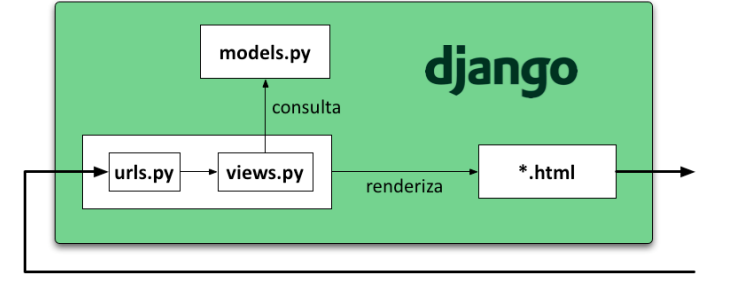
\includegraphics[width=12cm, keepaspectratio]{img/django.png}
    \caption{Estructura de Django}
    \label{fig:django}
\end{figure}

Los modelos en Django son objetos en Python que son guardados en una base de datos. Los modelos son independientes al gestor de base de datos que se vaya a utilizar, se definen las estructuras de información de una manera genérica y además se puede añadir restricciones. Django puede traducir filtros de python en SQL gracias a su ORM, por lo tanto no es necesario saber lenguaje de datos. Los modelos estan formado por una lista de campos donde se define el dominio de cada campo, si no hay ningún campo que tenga una clave primaria, Django generará una columna llamada id que se incrementará automáticamente. Los modelos se escriben en el fichero \textit{models.py}.\cite{model}\\

Las vistas en Django esta formado por el fichero \textit{urls.py} y \textit{views.py}. En el fichero\textit{ urls.py} a partir de expresiones regulares se definen las urls que redirigen a funciones de \textit{views.py.} La función \textit{views.py} recibe un objeto \textit{HTTP Request} y todos los parámetros de la URL capturados teniendo que devolver un objeto \textit{HTTP Response}. Lo habitual en web dinámicas es hacer una consulta a la base de datos, generar un contexto que empotra en una plantilla y a través la cual se renderiza devolviendo un HTTP Response.\\

Las plantillas son páginas dinámicas, es decir, son protopáginas la cuales solo se pueden renderizar juntando el contexto (diccionario con los valores que dan contexto a una plantilla) pasado por las vistas y gracias al lenguaje de plantillas dando como resultado normalmente un documento HTML. Esto es útil al programar ya que permite hacer páginas dinámicas en pocas líneas\\

En resumen para formar un servidor en Django primero hay que diseñar el modelo de datos, luego se diseñan las urls que enrutaran a las vistas las cuales preparan un contexto que juntándolo con la plantilla se genera el HTTP Response.\\

La versión actual de Unibotics está basada en Django 2.2.

\subsection{SQL}
SQL\footnote{Structured Query Language} es un lenguaje de de consulta estructurado, se utiliza para definir, manipular y gestionar los datos almacenados en una base de datos relacional. SQL es un estándar reconocido en 1986 por ANSI\footnote{American National Standards Institute} y en 1987 por ISO\footnote{International Organization for Standardization}\\

Se necesita un gestor de base de datos RDBMS\footnote{Relational Database Management System}  que se encargará de interactuar con la base de datos por ejemplo MySQL o  Access SQL. Algunos de estos gestores trabajan en local y otros en un servidor remoto.\cite{rdbms}\\

\begin{figure}[H]
    \centering
    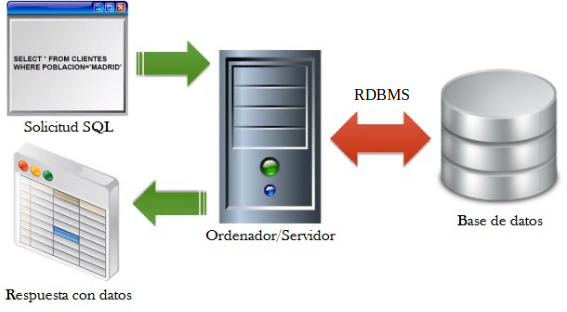
\includegraphics[width=11cm, keepaspectratio]{img/sql.png}
    \caption{Esquema funcionamiento SQL}
    \label{fig:sql}
\end{figure}
Una instrucción SQL esta formada por comandos, cláusulas, operadores y funciones . Los comandos de una sentencia SQL se dividen en cuatro tipos:
\begin{itemize}
\item DDL (\textit{Data Definition Language}): sirve para crear o modificar la estructura de una base de datos. Algunos de los camandos más importantes de este tipo son \textit{CREATE }para crear nuevas tablas o base de datos, \textit{ALTER} para modificar la tabla de la base de datos, \textit{DROP} para eliminar tablas o índices 
\item DML (\textit{Data Manipulation Language}): sirve para hacer consultas de selección y de acción a la base de datos. Por ejemplo tenemos los comandos \textit{SELECT} para extraer los datos,\textit{ INSERT} para insertar nuevos datos, UPDATE para actualizar los datos y \textit{DELETE} para eliminarlos.
\item DCL (\textit{Data Control Language}): se utiliza para proporcionar seguridad a la base de datos. El comando para otorgar permiso es \textit{GRANT} y para retirarlos es \textit{REVOKE}
\item TCL (\textit{Transactional Control Language}): su función es administrar los cambios en los datos. De este tipo de comandos se tiene \textit{COMMIT} para guardar el trabajo realizado o \textit{ROLLBACK} para deshacer las últimas modificaciones hechas después del último \textit{COMMIT}
\end{itemize}

Las cláusulas son condiciones de modificación para poder definir los datos. Las cláusulas más importantes son \textit{FROM} para especificar la tabla, \textit{WHERE} para definir las condiciones de los registros que se desean, \textit{GROUP BY} para hacer agrupaciones específicas de registros, \textit{HAVING} para declarar la condición que debe cumplir cada grupo, \textit{ORDER BY} para que los registros sigan un orden especificado.\\

Los operadores pueden ser lógicos, por ejemplo, \textit{AND}, \textit{OR} o \textit{NOT}) o de comparación que serían las operaciones del estilo mayor que, menor que o igual que. Las funciones se utilizan con el comando \textit{SELECT} para devolver un único valor de un grupo de registros como puede ser\textit{ AVG }que te devuelve la media o \textit{COUNT }para devolver el número de registros. En la figura \ref{fig:ejsql} se muestra un ejemplo de una sentencia SQL con con todas sus partes.\cite{sql}\\

\begin{figure}[H]
    \centering
    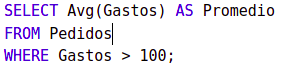
\includegraphics[width=9cm, keepaspectratio]{img/ejsql.png}
    \caption{Sentencia SQL}
    \label{fig:ejsql}
\end{figure}
En este TFG se ha utilizado SQL ya que Unibotics dispone de una base de datos MySQL donde se almacena la información estructural de la plataforma como los usuarios o ejercicios, a la cual se accede a través de Django.

\section{Recogida y grabación de datos}
Para la recogida y grabación de las sondas es necesario tener una base de datos, en este caso para este proyecto se ha decidido utilizar una base de datos no relacional (NoSQL\footnote{\textit{Not only SQ}L}). Una base de datos no relacional se caracteriza por almacenar datos no estructurados o semi-estructurados, además sus datos no están organizados en tablas como era el caso de las bases de datos relacionales por ejemplo MySQL.\\

En este TFG se ha utilizado Elasticsearch\footnote{https://www.elastic.co/}, el cual es un motor de búsqueda y análisis de código abierto, escrito en Java y basado en Lucene, una biblioteca de Java que proporciona funciones de indexación y búsqueda entre otras. Elasticsearch está orientado a documentos JSON\footnote{JavaScript Object Notation} formado por un conjunto de pares clave-valor, donde la clave es una cadena de texto y el valor puede ser de diferentes tipos como un texto o una lista.\cite{elastic}\\

Elasticsearch se caracteriza por ser una herramienta rápida permitiendo una búsqueda de texto completo bastante eficiente. Gracias al poco tiempo transcurrido entre la indexación (grabación de datos en Elasticsearch) y la posterior búsqueda hemos considerado que se trata de una herramienta adecuada para la grabación de las sondas y la posterior consulta de la información. Una de las ventajas de las bases de datos no relacionales es que están implementadas para permitir un escalado horizontal, es decir se puede dividir la base de datos en diferentes servidores, de una manera más sencilla que con las bases de datos relacionales. Los diferentes datos están agrupados en lo que se llama \textit{shards} en los cuales se aplican técnicas de réplica para ser tolerante a los fallos, además si Elasticsearch tiene algún fallo es capaz de detectarlo y reorganizar la información. Existen diferentes módulos en diferentes lenguajes de programación que permiten una interacción sencilla con Elasticsearch.\cite{elastic2}\\

Elasticsearch esta formado por \textit{clusters} que son un conjunto de nodos, en los cuales se almacena todos los datos, también puede estar formado por un único nodo. Al \textit{cluster} se le asigna un nombre y un identificador único. Los nodos que se encuentran en un \textit{cluster} son unos servidores únicos que almacenan documentos y ayuda en las capacidades de indexación del \textit{cluster}, al nodo también se le asigna un nombre y un identificador. Dentro de los nodos se pueden encontrar uno o más índices que son una colección de documentos con características similares, tiene que ser nombrado en minúsculas y será este nombre al que se hará referencia para realizar las diferentes operaciones. Los documentos que encontramos en un índice esta formada por la información básica que es recogida.\cite{elastic3}\\



\begin{figure}[H]
    \centering
    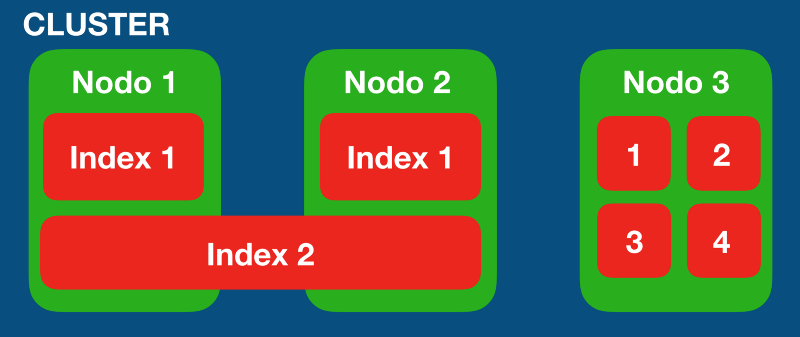
\includegraphics[width=12cm, keepaspectratio]{img/arquitectura_elastic.png}
    \caption{Arquitectura Elasticsearch}
    \label{fig:elastic}
\end{figure}
En el caso que se guarde una gran cantidad de documentos sobrepasando los límites de almacenamiento de un nodo, Elasticsearch divide cada índice en diferentes fragmentos (\textit{shards}), la distribución de cada fragmento por los diferentes nodos se realiza de forma automática. Para evitar fallos en los nodos se hacen réplicas de los \textit{shards} y se almacenan en un nodo diferente al \textit{shard} primario, así en el caso de que se produzca un fallo en un nodo se podrá seguir trabajando.\\

En este TFG se ha utilizado la versión 7.12.0 de Elasticsearch.
\newpage

\section{Visualización de estadísticas automática}

Una vez ya recogido las sondas y se han almacenado en Elasticsearch, es la hora de poder visualizarlos para poder hacer un análisis de los resultados. En este TFG se ha decidido utilizar el \textit{framework }Dash\footnote{https://dash.plotly.com/} para poder realizar esta tarea. Dash es un \textit{low-code framework}, es decir que permite la creación de aplicaciones de manera rápida y eficiente haciendo un menor uso de la programación manual, está escrito sobre Plotly.js y React.js. Dash está disponible en lenguajes de programación como Python, Julia, R o F#. Dash es multiplataforma, por lo que puede ser utilizado desde cualquier dispositivo.\cite{dash}\\

En las aplicaciones de dash no es necesario escribir ningún documento HTML, JavaScript o CSS ya que Dash proporciona una abstracción pura en Python mediante el uso de la biblioteca de \texttt{dash\_html\_components}. Otra biblioteca de python que se utiliza en una aplicación Dash es \texttt{dash-core-components} el cual son una serie de componentes para una interfaz de usuario interactiva como un menú desplegable.\\

La estructura de los datos que se van a visualizar en  Dash son\textit{ Dataframe} de la biblioteca de Pandas\footnote{Python Data Analysis Library}. Un DataFrame es una tabla en la que los datos guardados en cada columna representan las diferentes variables.\\

Las aplicaciones de Dash están formadas por dos partes la primera es la llamada \textit{layout} donde se describe cual va a ser el aspecto de la aplicación, esto son los menús y las gráficas que se visualizan, aquí es donde se utilizaran las bibliotecas mencionadas anteriormente. La segunda parte es la interactividad con los usuarios, para ello se utiliza \texttt{dash.dependencies} donde los componentes interactivos crean una entrada y a través de \textit{callbacks} modifican las gráficas, de tal manera que se pueden integrar filtros para generar diferentes visualizaciones en base a las necesidades del usuario.\\

Para este TFG se ha utilizado Dash en la versión 1.17.0.















